% \documentclass[handout,xcolor=pdftex,dvipsnames,table]{beamer}
\documentclass{beamer}

\usepackage{amsmath}
\usepackage[english,brazil]{babel}
\usepackage[utf8x]{inputenc}
\usepackage{graphicx}
\usepackage{url,color,ae}
\usepackage{listings,color,upquote}
\usepackage[T1]{fontenc}

\hypersetup{pdftitle={IFSC - Campus Sao Jose},
 	pdfsubject={Telecomunicacoes}
}



%--------- Insercao de codigo fonte nos slides --------------------%
\definecolor{hellgelb}{rgb}{1,1,0.9}
\definecolor{colKeys}{rgb}{0,0,0}
\definecolor{colIdentifier}{rgb}{0,0,0.9}
\definecolor{colComments}{rgb}{.4,.4,.4}
\definecolor{colString}{rgb}{0,0,0.6}

% Comando: \java
\newcommand{\java}
{\lstset{language=java,basicstyle=\ttfamily\footnotesize,tabsize=3,frame=single,showtabs=false,showspaces=false,firstnumber=last,numbers=left,numberstyle=\tiny,linewidth=0.98\linewidth,xleftmargin=21pt,tab=$\to$,float=tbph,extendedchars,breaklines,showstringspaces=false,identifierstyle=\color{colIdentifier},keywordstyle=\color{colKeys},stringstyle=\color{colString},commentstyle=\color{colComments},backgroundcolor=\color{hellgelb},columns=flexible,captionpos=b,aboveskip=\bigskipamount}}

% Comando: \shell
\newcommand{\shell}
{\lstset{language=csh,basicstyle=\ttfamily\footnotesize,tabsize=3,frame=single,showtabs=false,showspaces=false,firstnumber=last,numbers=left,numberstyle=\tiny,linewidth=0.98\linewidth,xleftmargin=21pt,tab=$\to$,float=tbph,extendedchars,breaklines,showstringspaces=false,identifierstyle=\color{colIdentifier},keywordstyle=\color{colKeys},stringstyle=\color{colString},commentstyle=\color{colComments},backgroundcolor=\color{hellgelb},columns=flexible,captionpos=b,aboveskip=\bigskipamount}}

% ------------------ TEMA ---------------------------------------------%

\usetheme[numbers,totalnumber,compress]{Madrid}
% \usetheme{Warsaw}
% \usetheme{Boadilla}
% \usetheme{CambridgeUS}
% \usetheme{Montpellier}
% \usetheme{Hannover}
% \usetheme{Dresden}

\definecolor{azulescuro}{rgb}{0.3,0.42,0.601}  
\definecolor{verde}{rgb}{0.55,0.78,0.25} 
\definecolor{kugreen}{RGB}{50,93,61}
\definecolor{kugreenlys}{RGB}{132,158,139}
\definecolor{kugreenlyslys}{RGB}{173,190,177}
\definecolor{kugreenlyslyslys}{RGB}{214,223,216}
 
\usecolortheme[named=kugreen]{structure}
\useinnertheme{circles}

\setbeamertemplate{footline}[frame number]
\beamertemplatenavigationsymbolsempty
% ------------------------------------------------------------------ %

\logo{
\includegraphics[width=.5cm]{logo-ifsc}}






% -------------------- Titulo -----------------------------------%

\title{Título da aula}
\subtitle{Redes Multimídia}
\author[Prof. Emerson Mello]{Prof. Emerson Ribeiro de Mello}
\institute[IFSC]{
Instituto Federal de Santa Catarina -- IFSC\\
campus São José \\
\url{mello@ifsc.edu.br}
}

\date{janeiro de 2011}


% -------------- Início do documento ------------------ %
\begin{document}

\begin{frame}
	\maketitle
\end{frame}

\frame{\frametitle{Conteúdo programático}
\tableofcontents}

\AtBeginSection[]{
  \frame{
    \frametitle{Conteúdo programático}
    \tableofcontents[current,currentsection]
  }
}

\section{Conceitos sobre segurança em redes}

\begin{frame}
	\frametitle{Propriedades básicas de segurança}
	A segurança está fundamentada sobre três propriedades básicas:\\
	\begin{itemize}
		\item \textbf{Confidencialidade} -- A informação só deve ser revelada para usuários autorizados a acessá-la
		\item \textbf{Integridade} -- A informação não poderá ser modificada, intencionalmente ou acidentalmente, por usuários que não possuam direito para tal
		\item \textbf{Disponibilidade} -- O uso do sistema não poderá ser negado, de forma maliciosa, aos usuários autorizados
	\end{itemize} 
\end{frame}

\frame{
	\frametitle{Vulnerabilidades, ameaças e ataques}
	\begin{itemize}[<+->]
		\item \textbf{Vulnerabilidades} -- Um erro de programação, erro na configuração ou mesmo um erro de operação
		\item \textbf{Ameaças} --  possível ação que, se concretizada, poderá produzir efeitos indesejados ao sistema, comprometendo as propriedades básicas de segurança
		\item \textbf{Ataques} -- é a concretização de uma \textbf{ameaça}, explorando alguma \textbf{vulnerabilidade} do sistema, executado por algum intruso, de forma maliciosa ou não
	\end{itemize} 
}

\frame{
	\frametitle{Medidas de segurança}
	\begin{itemize}
		\item<1-> \textbf{Prevenção} -- Significa que um ataque irá falhar.
		\begin{itemize}
			\item<1-> Implica no uso de mecanismos de segurança que não podem ser ignorados -- Ex: uso de senhas
		\end{itemize} 
		\item<2-> \textbf{Detecção} -- Quando um ataque não pode ser prevenido
		\begin{itemize}
			\item<2-> informa que um ataque está em andamento ou que ocorreu 
			\begin{itemize}
			\item<2-> Ex: monitoramento das tentativas de logins, Sistema de detecção à Intrusão (\textit{IDS}) 
			\end{itemize} 
		\end{itemize} 
		\item<3-> \textbf{Recuperação} -- Existem duas formas
		\begin{itemize}
			\item<3-> Interrompe o ataque e repara o dano
			\begin{itemize}
				\item<3-> Ex: cópia de segurança de um arquivo que foi excluído
			\end{itemize} 
			\item<3-> Repara o dano com o sistema em funcionamento e com o ataque em andamento
			\begin{itemize}
				\item<3-> Ex: tolerância à falta
			\end{itemize} 
		\end{itemize} 
	\end{itemize} 
}

\section{Conceitos sobre Firewall}

\frame{
	\frametitle{Firewall}
	\begin{block}{Definição convencional: Parede corta fogo}
		Dispositivo feito de material a prova de fogo para evitar que o fogo se espalhe de uma parte do edifício para outra
	\end{block}
	\pause
	\begin{block}{Definição para sistemas computacionais}
	 Ponto de controle que mantém acessos não autorizados fora do perímetro de segurança, ao mesmo tempo possibilita acesso aos sistemas externos
	\end{block}
	\begin{itemize}
		\item Atua como uma barreira de segurança entre a rede interna e o mundo exterior
		\item Evita que potenciais vulnerabilidades de serviços sejam exploradas
		\begin{itemize}
			\item Nenhum software complexo é 100\% seguro
		\end{itemize}
		\item Pode ser classificado como firewall de \textbf{máquina} ou de \textbf{rede}
	\end{itemize} 
}

\frame{
	\frametitle{Firewall de rede}
	\begin{itemize}
		\item \textbf{Perímetro de segurança:} rede local da organização
		\item Todo o tráfego de dentro para fora, e vice-versa, deverá passar pelo \textit{Firewall}
		\item Somente o tráfego autorizado, definido pela política de segurança local, deverá ter permissão para passar
		\item O próprio \textit{Firewall} deverá ser imune a invasões
		\begin{itemize}
			\item Implica na utilização de um sistema confiável, com um sistema operacional seguro e rodando um conjunto mínimo de serviços
		\end{itemize} 
	\end{itemize} 
	\begin{figure}
	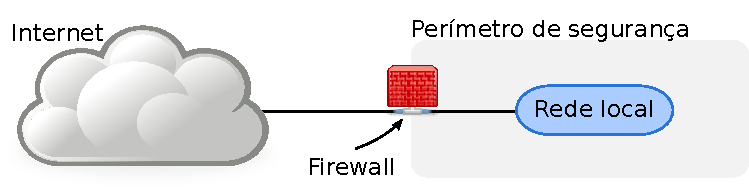
\includegraphics[scale=.8]{figs/firewall}
	\end{figure}
}

\section{Projetos de firewall}

\subsection{Perímetros de segurança}

\begin{frame}
	\frametitle{Organização da rede}
	\begin{columns}

		\column{.5\linewidth}

	\begin{enumerate}
		\item<1-|alert@1> \textbf{Somente com estações de trabalho}
		\begin{itemize}
			\item<1-|alert@1> Residencias e pequenas empresas
		\end{itemize}
		\item<2-|alert@2> \textbf{Estações e servidores internos}
		\begin{itemize}
			\item<2-|alert@2> Servidor de impressão, arquivos, etc.
		\end{itemize}
		\item<3-|alert@3> \textbf{Estações, servidores internos e externos}
		\begin{itemize}
			\item<3-|alert@3> WWW, SMTP, DNS, POP, IMAP, etc.
		\end{itemize}
	\end{enumerate}

	\column{.5\linewidth}

	\begin{center}
	 \only<1|handout:0>{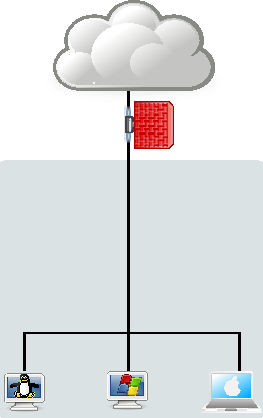
\includegraphics[scale=.8]{figs/organizacao-redes1}}%
	 \only<2|handout:0>{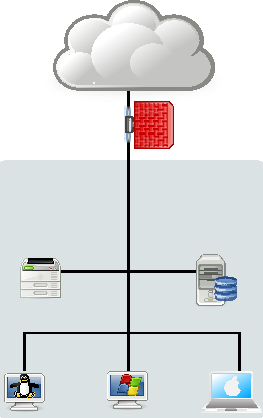
\includegraphics[scale=.8]{figs/organizacao-redes2}}%
	 \only<3-|:handout:1>{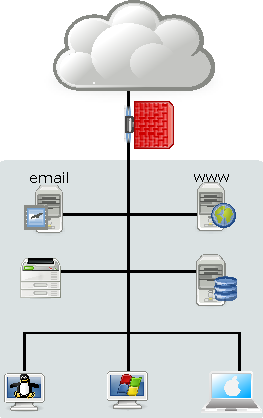
\includegraphics[scale=.8]{figs/organizacao-redes3}}%
	\end{center}
	\end{columns}
	\visible<4|handout:1>{
	\begin{block}{}
		Como oferecer serviços externos sem que isto resulte em ameaças para a rede interna?
	\end{block}}
\end{frame}

\section{Códigos embutidos}



\java

\begin{frame}[fragile]
	\frametitle{Código em Java}	
	\begin{itemize}
		\item Lembre-se de colocar a opção \textbf{fragile} no frame.
	\end{itemize}
	\begin{lstlisting}
	 public class Ola{
	   public void olaMundo(){
	      System.out.println("Ola mundo!");
	   }
	 }
	\end{lstlisting}
\end{frame}

\shell

\begin{frame}[fragile]
	\frametitle{Código em Shell Script}	
	\begin{itemize}
		\item Lembre-se de colocar a opção \textbf{fragile} no frame.
	\end{itemize}
	\begin{lstlisting}
	 echo "ola mundo"
	\end{lstlisting}
\end{frame}


\begin{frame}
	\frametitle{Bibliografia}
	\begin{thebibliography}{1}
	\beamertemplatebookbibitems

  \bibitem{stallings}
    William Stallings
    \newblock {\em Network Security Essentials}.
    \newblock Prentice Hall, 2000.

  \bibitem{bishop}
    Matt Bishop
    \newblock {\em Computer Security -- Art and Science}.
    \newblock Addison Wesley, 2003.

  \bibitem{pfleeger}
    Charles P. Pfleeger and Shari Lawrence Pfleeger
    \newblock {\em Security in Computing}.
    \newblock Prentice Hall, 2006.

 	\beamertemplatearticlebibitems

	\bibitem{rfc2196}
	B. Fraser
	\newblock {\em Site Security Handbook}.
	\newblock RFC 2196, 1997.

	\end{thebibliography}
\end{frame}










\end{document}
